\documentclass[11pt]{article}
\usepackage[T1]{fontenc}	%special characters
\usepackage[utf8]{inputenc}	%special characters
\usepackage{lmodern,textcomp}% Euro Symbol

\usepackage{hyperref}
\usepackage[margin=1in]{geometry} %article layout margins
\usepackage{tabularx}		%tabulars width fixed textwidth
\usepackage{multicol}	%2 columns in Skills
\usepackage{graphicx}
\usepackage{sectsty}
\sectionfont{
	\sectionrule{0pt}{0pt}{-5pt}{0.8pt}
}

\begin{document}

\Large
\noindent
\textbf{Dirk Hornung, Ph.D.} \\

\normalsize
\noindent
\begin{minipage}{0.5\linewidth}
  \begin{tabularx}{0.6\textwidth}{>{\bfseries}l l}
    City:           & Barcelona \\
    Date of birth:  & October 5, 1991\\
    Place of birth: & Fulda, Germany \\
    Mobile:         & +34 695460404 \\
    E-mail:         & hello@drdirk.io \\
    Website:      	& drdirk.io
  \end{tabularx}
\end{minipage}
\begin{minipage}{0.5\linewidth}
  \begin{flushright}
    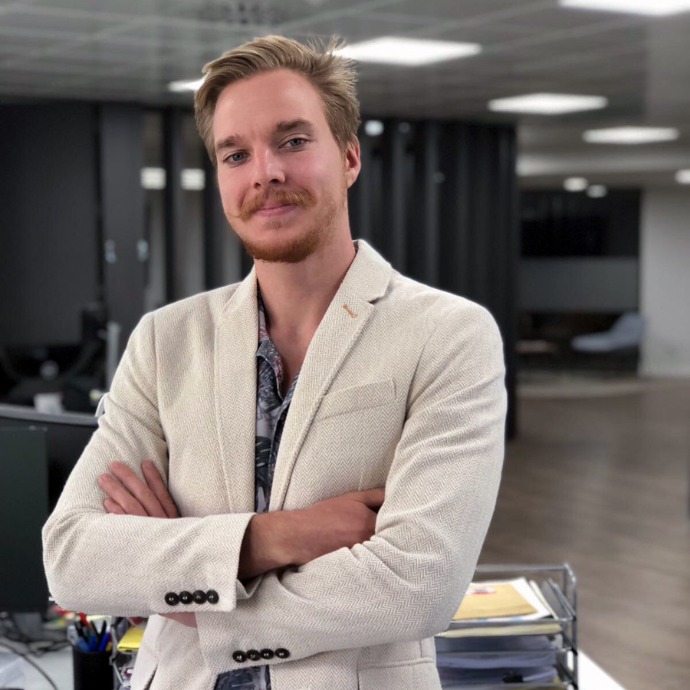
\includegraphics[width=0.4\textwidth]{dirk.png}
  \end{flushright}
\end{minipage}

\section*{}
\vspace{0.5cm}
Warum ich perfekt in das Gardena Team bei Husqvarna passe. \\

\noindent Ich heiße Dirk Hornung, bin gebürtiger deutscher und lebe seit 5 Jahren in
Spanien. Ich habe in diesem Jahr meine Promotion in der theoretischen
Teilchenphysik erfolgreich abgeschlossen und suche nun nach neuen
Herausforderungen.

\noindent Seit meinem 14. Lebensjahr verbringe ich einen Großteil meiner Zeit mit der
Programmierung von Applikationen. Mit jedem Projekt versuche ich neue
Technologien zu erlernen. Ich stufe mich als erfahrenen Full-Stack
Developer mit Kenntnissen in der Blockchain und der künstlichen
Intelligenz ein. Mein Schwerpunkt ist die Frontendentwicklung, am
liebsten in Typescript mit React und Mocha.

\noindent Seit Beginn letzten Jahres habe ich mir, passend zu Ihren Smart Garden
Robotern, einen Makerspace eingerichtet. Der Makerspace besteht aus einem 3D
Drucker, einer CNC-Fräse und unzähligen Hardwarekomponenten und wurde von mir
verwendet um mir ein Smart Home einzurichten und in die Elektrotechnik
einzusteigen.

\noindent Ich habe lange Zeit für Early-Stage Startups gearbeitet und suche nun
ein international anerkanntes Unternehmen, wie Husqvarna, um meine Karriere
voranzutreiben. Ich möchte in der Frontentwicklung arbeiten, weil ich dort die
meiste Erfahrung mitbringe und zusätzlich diese Erfahrung in meinem CV
ausbauen. Das Gardena-Team, Smart-Home und IoT hören sich nach einem
interessanten Arbeitsfeld an, indem es viel zu lernen gibt. Zudem sind meine
Freundin und ich unzufrieden mit unserer Lebensqualität in Spanien. Wir suchen
daher einen Neustart in der Schweiz.

\noindent Warum eigne ich mich besonders für die Stelle? Ich bringe viele Jahre
Erfahrung als Frontendentwickler in Frameworks wie React und Angular mit. Ich
bin überzeugt von der Wichtigkeit von Unit-Tests. Mit meinem Doktortitel und
vielseitigen Interessen dürfte ich eine Besonderheit in der
Frontendentwicklung sein. Zudem habe gute soziale Kompetenzen, 
ausgezeichnete Kommunikationsfähigkeiten und bin ein passionierter Lehrer. \\

\noindent Ich hoffe Ich konnte Sie von mir überzeugen und freue mich auf Ihre
Rückmeldung. \\

\noindent Mit freundlichen Grüßen, Dr. Dirk Hornung \\

\noindent P.S. Ich habe mir letzten einen Putzroboter gekauft und versuche seit
geraumer Zeit (erfolglos) die Mutter meiner Freundin für den Kauf eines automatischen
Rasenmähers zu gewinnen.

 \end{document}